\documentclass{beamer}

\usepackage{tikz}
\usetikzlibrary{shapes.multipart}

\usepackage[dvipsnames]{xcolor}

%Information to be included in the title page:
\title{Understanding the Structure of District Heating Networks from Measurement Data}
\subtitle{A First Overview}
\author{Fabian Weik}
\institute{Fraunhofer ITWM}
\date{\today}

\begin{document}

\frame{\titlepage}

\begin{frame}
\frametitle{Motivation}
  \begin{itemize}
    \item Sometimes, the information about the structure of district heating networks is incomplete
    \item But needed for precise simulation
  \end{itemize}

  \vspace{2em}

  To be determined
  \begin{itemize}
    \item What information is provided
    \item How to complete that information using measurement data
  \end{itemize}
\end{frame}

\begin{frame}
\frametitle{Influence of the Structure (Current Procedure)}
  \begin{figure}
    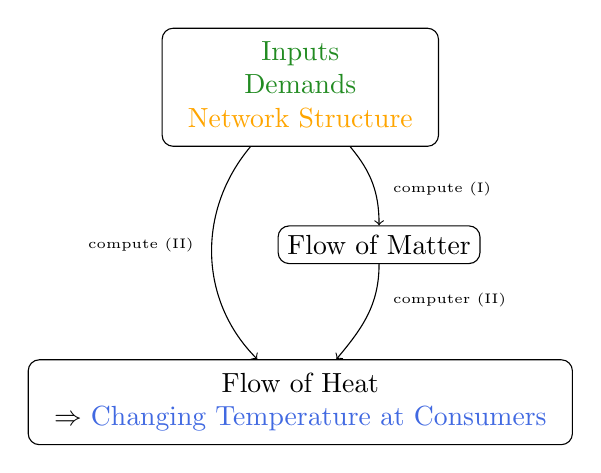
\begin{tikzpicture}
      \node (A) [rectangle, draw, rounded corners] at (0, 2) {
        \begin{tabular}{c}
          \color{ForestGreen}
          Inputs \\
          \color{ForestGreen}
          Demands \\
          \color{Orange}
          Network Structure
        \end{tabular}
      };
      \node (B) [rectangle, draw, rounded corners] at (1, 0) {
        Flow of Matter
      };
      \node (C) [rectangle, draw, rounded corners] at (0, -2) {
        \begin{tabular}{c}
          Flow of Heat \\
          $\Rightarrow$ \color{RoyalBlue} Changing Temperature at Consumers
        \end{tabular}
      };

      \draw[->] (A) to [out=310, in=90] (B) node [midway, right, xshift=30, yshift=20] {\tiny{compute (I)}};
      \draw[->] (A) to [out=230, in=135] (C) node [midway, left, xshift=-35] {\tiny{compute (II)}};
      \draw[->] (B) to [out=270, in=50] (C) node [midway, right, xshift=30, yshift=-20] {\tiny{computer (II)}};
    \end{tikzpicture}
  \end{figure}

  Computation split for efficiency
\end{frame}

\begin{frame}
\frametitle{Influence of the Structure}
  Simplify to (hopefully) allow backwards computation

  \vspace{2em}

  \begin{figure}
    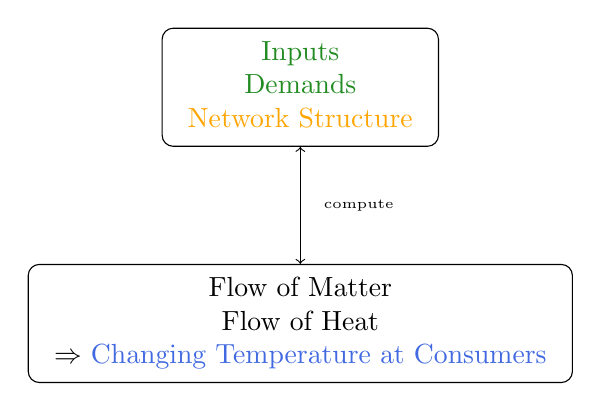
\begin{tikzpicture}
      \node (A) [rectangle, draw, rounded corners] at (0, 1.5) {
        \begin{tabular}{c}
          \color{ForestGreen}
          Inputs \\
          \color{ForestGreen}
          Demands \\
          \color{Orange}
          Network Structure
        \end{tabular}
      };
      \node (B) [rectangle, draw, rounded corners] at (0, -1.5) {
        \begin{tabular}{c}
          Flow of Matter \\
          Flow of Heat \\
          $\Rightarrow$ \color{RoyalBlue} Changing Temperature at Consumers
        \end{tabular}
      };

      \draw[<->] (A) to (B) node [midway, right, xshift=5] {\tiny{compute}};
    \end{tikzpicture}
  \end{figure}
\end{frame}

\begin{frame}
\frametitle{Finding Parameters --- A Proposal}
  \begin{itemize}
    \item Possible Connections as parameters
      \begin{itemize}
        \item Single values of edge icidence matrix
        \item Influences loop incidence matrix also
      \end{itemize}
    \item Optimize for low error
  \end{itemize}
\end{frame}

\end{document}
